\section{Ngữ liệu huấn luyện}
\subsection{Pretraining}
ViHealthBERT sử dụng các bộ ngữ liệu \textit{Text Mining Corpus} và \textit{OSCAR} cho quá trình pretraining. Vì sử dụng trọng số huấn luyện của PhoBERT nên các bộ ngữ liệu pretraining của PhoBERT cũng được đề cập trong bảng thông số các bộ ngữ liệu pretraining (bảng~\ref{tab:pretraining-stats}).

\begin{table}
\centering
\begin{tabular}{|l|c|c|}
\hline
\textbf{Dataset} & \textbf{\# Sent} & \textbf{Domain} \\ \hline
Vietnamese Wikipedia & 5M & General \\ \hline
Vietnamese news & 96M & General \\ \hline
Text Mining Corpus & 4.7M & Health, Medical \\ \hline
OSCAR's selected corpus (TF) & 25M  & Health, Medical, General \\ \hline
\end{tabular}
\caption{Thông số các bộ ngữ liệu pretraining\cite{minh-EtAl:2022:LREC}}
\label{tab:pretraining-stats}
\end{table}

\subsubsection{Text Mining Corpus}
Để xây dựng bộ ngữ liệu \textit{Text Mining Corpus}, nhóm tác giả thu thập ngữ liệu từ các trang tin điện tử, các website bệnh viện, tạp chí khoa học và sách chuyên khảo về y khoa:
\begin{itemize}
\item \textbf{Các trang tin điện tử / website bệnh viện}: nhóm tác giả dùng các từ khóa liên quan đến "y học", "vắc-xin", "y sinh" hay "sức khỏe" để tìm các website liên quan đến chủ đề y tế.
\item \textbf{Các tạp chí khoa học}: nhóm tác giả trích xuất phần tóm tắt (abstract) của các tạp chí Vietnamese Medical Journal, Journal of Health and Development Studies, Journal of Medicine and Pharmacy, Medical Journal of Ho Chi Minh City.
\item \textbf{Sách chuyên khảo}: nhóm tác giả dùng bản pdf sách chuyên khảo y sinh từ website \texttt{yhoctonghop.vn}, sau đó chuyển bản pdf sang phiên bản text.
\end{itemize}
Phần ngữ liệu thô được tiền xử lý (preprocess) với các bước khử nhiễu; loại bỏ địa chỉ email, số điện thoại, URL trong văn bản; loại bỏ các câu trùng lặp bằng khoảng cách Levenshtein.

\subsubsection{OSCAR's selected corpus}
Để xây dựng Bộ ngữ liệu OSCAR\cite{ortiz-suarez-etal-2020-monolingual}, nhóm tác giả đã dùng các phương pháp \textbf{Term Frequency (TF)} và \textbf{Selector} vì bộ ngữ liệu OSCAR là bộ ngữ liệu cho general-domain, trong khi ta chỉ cần trích xuất các văn bản liên quan đến chủ đề y tế.

\paragraph{Term Frequency (TF)}
Phương pháp Term Frequency dựa vào tần suất xuất hiện của các từ liên quan đến chủ đề y tế để xác định xem một văn bản có thuộc chủ đề y tế hay không. Các bước thực hiện bao gồm:
\begin{enumerate}
\item Dựng một từ điển với bộ ngữ liệu thu thập được.
\item Chọn 3000 từ xuất hiện trên 10000 lần liên quan tới chủ đề y tế. Thao tác có sự kiểm tra của chuyên gia để đảm bảo các từ khóa thực sự liên quan tới chủ đề y tế.
\end{enumerate}

\paragraph{Selector}
SimCSE (\textbf{Sim}ple \textbf{C}ontrastive Learning of \textbf{S}entence \textbf{E}mbeddings)\cite{simcse2021} là một phương pháp sentence embedding hiệu quả dựa trên kiến trúc BERT, đạt những kết quả đáng chú ý với task Semantic Textual Similarity (STS)\footnote{Vì nội dung tìm hiểu xoay quanh mô hình ViHealthBERT nên nhóm chỉ tập trung vào ứng dụng của SimCSE trong toàn bộ nghiên cứu. Về chi tiết mô hình SimCSE, xin tham khảo \href{https://arxiv.org/abs/2104.08821}{https://arxiv.org/abs/2104.08821}}. Nhóm tác giả chọn ra một tập ngữ liệu mẫu từ các nguồn Vietnamese News Corpus và bộ Text Mining Corpus bên trên, sau đó chia tập ngữ liệu thành 2 phần: 
\begin{itemize}
\item Tập \textit{train-unsup} để huấn luyện một Encoder ánh xạ các câu văn vào không gian vector.
\item Tập \textit{train-sup} để huấn luyện một bộ phân lớp (classifier) từ các vector đầu ra của Encoder.
\end{itemize}
Bộ phân lớp SimCSE sau khi huấn luyện có thể xác định xem một văn bản có liên quan tới chủ đề y tế hay không. Dựa trên bộ phân lớp này, nhóm tác giả tiến hành trích xuất các văn bản liên quan đến chủ đề y tế từ các bộ ngữ liệu lớn hơn.

\subsection{Downstream task datasets}
Nhóm tác giả xây dựng các bộ ngữ liệu \textit{arcDrAid} và \textit{Frequently Asked Question (FAQ) Summarization} cho các downstream task:
\begin{itemize}
\item Acronym Disambiguation \textit{(Phân định từ viết tắt)}: xác định cụm từ đầy đủ của một từ viết tắt trong một ngữ cảnh nhất định. (e.g. \textit{vctc} có thể là \textit{viêm cổ tử cung} hoặc \textit{viêm cầu thận cấp}, tùy vào ngữ cảnh)
\item FAQ Summarization \textit{(Tóm tắt câu hỏi y tế)}: tóm tắt một câu hỏi / văn bản liên quan đến chủ đề y tế mà vẫn giữ nguyên ý nghĩa, độ khó và những thông tin quan trọng.
\end{itemize}

\begin{figure}
\centering
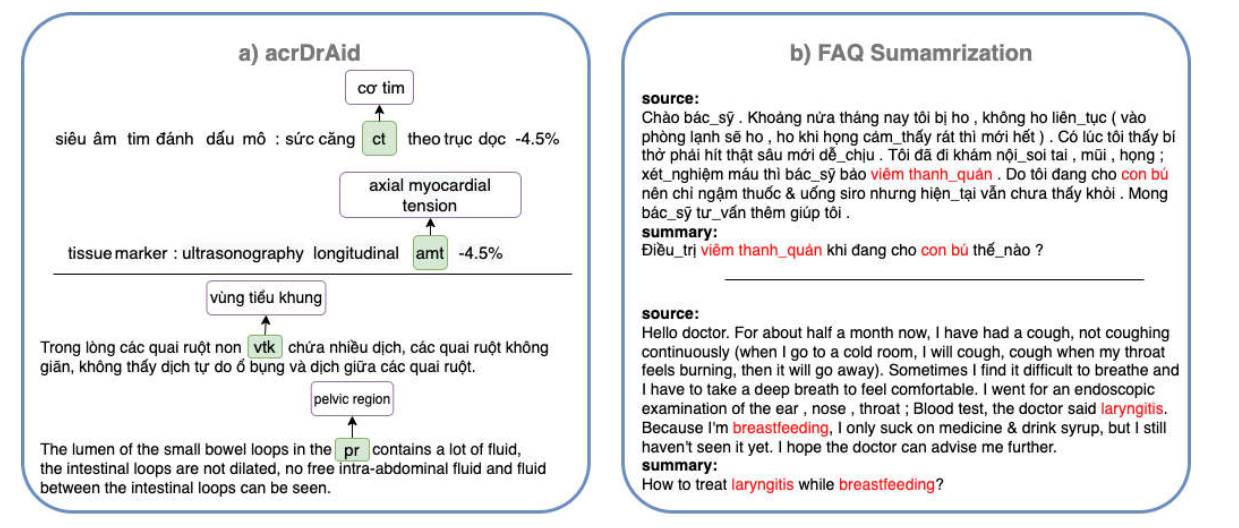
\includegraphics[scale=.65]{img/finetune-datasets.PNG}
\caption{Ví dụ cho tập ngữ liệu a) arcDrAid và b) FAQ Summarization\cite{minh-EtAl:2022:LREC}}
\label{fig:finetune-datasets}
\end{figure}

\subsubsection{arcDrAid}
Nhóm tác giả tiến hành xây dựng bộ ngữ liệu arcDrAid dựa trên các chẩn đoán hình ảnh từ bệnh viện Vinmec, dựa trên thực tế là các bác sĩ chẩn đoán hình ảnh thường viết tắt các triệu chứng bệnh lí để tiết kiệm thời gian. Quá trình xây dựng bộ ngữ liệu được thực hiện theo các bước sau:
\begin{enumerate}
\item Sử dụng công cụ POS-tagger của nhóm Underthesea\footnote{\href{https://github.com/undertheseanlp}{https://github.com/undertheseanlp}}, nhóm tác giả trích xuất ra 75000 cụm danh từ, sau đó chọn ra 1000 cụm danh từ có tần suất xuất hiện cao nhất.
\item Nhóm tác giả sử dụng các chữ cái đầu của mỗi âm tiết ghép lại tạo thành từ viết tắt cho một cụm danh từ (e.g. \textit{cơ tim} thành \textit{ct}). Các từ viết tắt chỉ đại diện cho một cụm danh từ duy nhất bị loại bỏ.
\item Các cụm từ được kiểm tra lại bởi chuyên gia để đảm bảo chúng thuộc chủ đề y tế.
\end{enumerate}
Bộ ngữ liệu được chia ngẫu nhiên thành các tập train/dev/test theo tỉ lệ 7/1/2. Các thông số của bộ ngữ liệu được trình bày trong bảng~\ref{tab:arcdraid-stats}
\begin{table}
\centering
\begin{tabular}{|p{3.75cm}|c|c|c|}
\hline
\textbf{Properties} & \textbf{Train} & \textbf{Dev} & \textbf{Test} \\ \hline
no. samples & 4000 & 523 & 1130 \\ \hline
average input length & 30.52 & 29.92 & 32.23 \\ \hline
no. unique acronym & 109 & 109 & 135 \\ \hline
average no. expansion per acronym & 3.16 & 3.19 & 3.04 \\ \hline
no. of unique expansion & 276 & 182 & 279 \\ \hline
average acronym expansion length & 2.064 & 2.064 & 2.067 \\ \hline
prob. overlap acronym over train set & 100\% & 100\% & 80.74\% \\ \hline
prob. overlap expansion over train set & 100\% & 97.8\% & 77.06\% \\ \hline
\end{tabular}
\caption{Thông số của bộ ngữ liệu arcDrAid\cite{minh-EtAl:2022:LREC}}
\label{tab:arcdraid-stats}
\end{table}

\subsubsection{FAQ Summarization}
Bộ ngữ liệu FAQ Summarization được xây dựng từ các website hỏi đáp (Q\&A) về sức khỏe, theo đó nhóm tác giả sử dụng tiêu đề của câu hỏi làm câu tóm tắt cho nội dung câu hỏi. Bộ ngữ liệu được chia theo tỉ lệ train/dev/test là 8/1/1. Các thông số của tập ngữ liệu FAQ Summarization được thể hiện trong bảng~\ref{tab:faq-summarization-stats}

\begin{table}
\centering
\begin{tabular}{|p{3.75cm}|c|c|c|}
\hline
\textbf{Properties} & \textbf{Train} & \textbf{Dev} & \textbf{Test} \\ \hline
no. samples & 10621 & 1326 & 1330 \\ \hline
avg. input length (word-level) & 93.3 & 90.28 & 94.01 \\ \hline
avg. input length (sentence-level) & 5.39 & 5.22 & 5.4 \\ \hline
avg. summary length (word-level) & 9.8 & 10.07 & 9.88 \\ \hline
avg. summary length (sentence-level) & 1.02 & 1.02 & 1.04 \\ \hline
prob. target token is included in input & 77.7\% & 78.17\% & 71.81\% \\ \hline
\end{tabular}
\caption{Thông số của bộ ngữ liệu FAQ Summarization\cite{minh-EtAl:2022:LREC}}
\label{tab:faq-summarization-stats}
\end{table}

\subsubsection{Các bộ ngữ liệu khác}
Nhóm tác giả sử dụng một số bộ ngữ liệu đã công bố cho task NER, bao gồm
\begin{itemize}
\item \textbf{PhoNER\_COVID-19\cite{truong-etal-2021-covid}}: bộ ngữ liệu gồm 10 loại thực thể, 10027 mẫu huấn luyện. Số mẫu của mỗi tập train/dev/test là 5027/200/3000.
\item \textbf{Vietnamese Medical Question (ViMQ)\cite{vimq-2021}}: bộ ngữ liệu gồm 3 loại thực thể, được chia thành 3 tập train/dev/test với số lượng mẫu mỗi tập lần lượt là 7000/1000/1000.
\end{itemize}